\documentclass[aspectratio=169]{beamer}
\usetheme{Madrid}
\usecolortheme{default}

\usepackage{graphicx}
\usepackage{caption}

% Set title and author
\title{Acceptance Discrepancy Investigation}
\subtitle{Comparing E906 Acceptance Calculations}
\author{Chatura Kuruppu}
\institute{Fermilab / NMSU}
\date{\today}

\begin{document}

% Title Slide
\begin{frame}
    \titlepage
\end{frame}

% Slide 1: Initial Discrepancy Overview
\begin{frame}{Initial Discrepancy: Overall Acceptance}
    \begin{columns}
        \column{0.5\textwidth}
        \centering
        \textbf{Chatura's Acceptance} \\
        \vspace{0.2cm}
        % Adjust the path or extension if necessary
        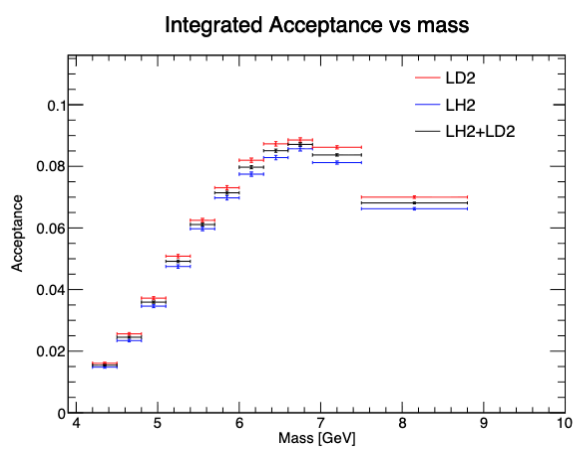
\includegraphics[width=0.95\textwidth]{acceptance_mass_chatura.png}
        
        \column{0.5\textwidth}
        \centering
        \textbf{Kenichi's Acceptance} \\
        \vspace{0.2cm}
        % Adjust the path or extension if necessary
        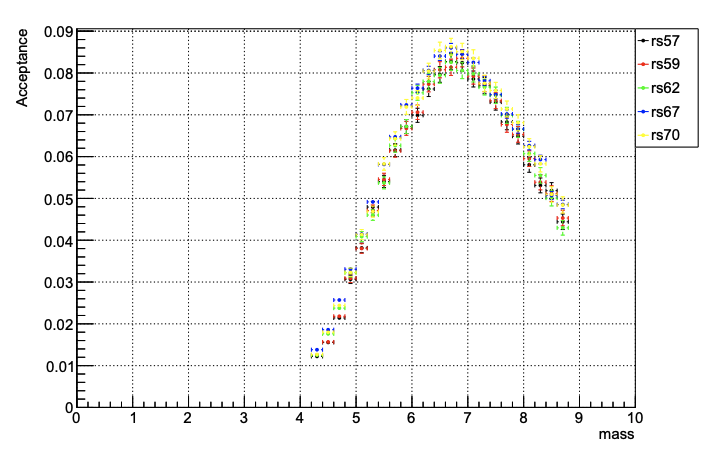
\includegraphics[width=0.95\textwidth]{acceptance_mass_kenichi.png}
    \end{columns}
    \vspace{0.5cm}
    \begin{itemize}
        \item Comparing the newly calculated acceptance to Kenichi's recent ROOT files.
        \item Next slides breakdown the discrepancy by $x_F$ bins (Hugo vs. No D1 Cut vs. With D1 Cut).
    \end{itemize}
\end{frame}

% Slide for xF bin 0
\begin{frame}{Acceptance Comparison: $x_F$ Bin 0}
    \begin{columns}
        \column{0.5\textwidth}
        \centering
        \textbf{LH2 Target} \\
        \includegraphics[width=\textwidth]{acceptance_comparisons/compare_LH2_xFbin0.pdf}
        
        \column{0.5\textwidth}
        \centering
        \textbf{LD2 Target} \\
        \includegraphics[width=\textwidth]{acceptance_comparisons/compare_LD2_xFbin0.pdf}
    \end{columns}
\end{frame}

% Slide for xF bin 1
\begin{frame}{Acceptance Comparison: $x_F$ Bin 1}
    \begin{columns}
        \column{0.5\textwidth}
        \centering
        \textbf{LH2 Target} \\
        \includegraphics[width=\textwidth]{acceptance_comparisons/compare_LH2_xFbin1.pdf}
        
        \column{0.5\textwidth}
        \centering
        \textbf{LD2 Target} \\
        \includegraphics[width=\textwidth]{acceptance_comparisons/compare_LD2_xFbin1.pdf}
    \end{columns}
\end{frame}

% Slide for xF bin 2
\begin{frame}{Acceptance Comparison: $x_F$ Bin 2}
    \begin{columns}
        \column{0.5\textwidth}
        \centering
        \textbf{LH2 Target} \\
        \includegraphics[width=\textwidth]{acceptance_comparisons/compare_LH2_xFbin2.pdf}
        
        \column{0.5\textwidth}
        \centering
        \textbf{LD2 Target} \\
        \includegraphics[width=\textwidth]{acceptance_comparisons/compare_LD2_xFbin2.pdf}
    \end{columns}
\end{frame}

% Slide for xF bin 3
\begin{frame}{Acceptance Comparison: $x_F$ Bin 3}
    \begin{columns}
        \column{0.5\textwidth}
        \centering
        \textbf{LH2 Target} \\
        \includegraphics[width=\textwidth]{acceptance_comparisons/compare_LH2_xFbin3.pdf}
        
        \column{0.5\textwidth}
        \centering
        \textbf{LD2 Target} \\
        \includegraphics[width=\textwidth]{acceptance_comparisons/compare_LD2_xFbin3.pdf}
    \end{columns}
\end{frame}

% Slide for xF bin 4
\begin{frame}{Acceptance Comparison: $x_F$ Bin 4}
    \begin{columns}
        \column{0.5\textwidth}
        \centering
        \textbf{LH2 Target} \\
        \includegraphics[width=\textwidth]{acceptance_comparisons/compare_LH2_xFbin4.pdf}
        
        \column{0.5\textwidth}
        \centering
        \textbf{LD2 Target} \\
        \includegraphics[width=\textwidth]{acceptance_comparisons/compare_LD2_xFbin4.pdf}
    \end{columns}
\end{frame}

% Slide for xF bin 5
\begin{frame}{Acceptance Comparison: $x_F$ Bin 5}
    \begin{columns}
        \column{0.5\textwidth}
        \centering
        \textbf{LH2 Target} \\
        \includegraphics[width=\textwidth]{acceptance_comparisons/compare_LH2_xFbin5.pdf}
        
        \column{0.5\textwidth}
        \centering
        \textbf{LD2 Target} \\
        \includegraphics[width=\textwidth]{acceptance_comparisons/compare_LD2_xFbin5.pdf}
    \end{columns}
\end{frame}

% Slide for xF bin 6
\begin{frame}{Acceptance Comparison: $x_F$ Bin 6}
    \begin{columns}
        \column{0.5\textwidth}
        \centering
        \textbf{LH2 Target} \\
        \includegraphics[width=\textwidth]{acceptance_comparisons/compare_LH2_xFbin6.pdf}
        
        \column{0.5\textwidth}
        \centering
        \textbf{LD2 Target} \\
        \includegraphics[width=\textwidth]{acceptance_comparisons/compare_LD2_xFbin6.pdf}
    \end{columns}
\end{frame}

% Slide for xF bin 7
\begin{frame}{Acceptance Comparison: $x_F$ Bin 7}
    \begin{columns}
        \column{0.5\textwidth}
        \centering
        \textbf{LH2 Target} \\
        \includegraphics[width=\textwidth]{acceptance_comparisons/compare_LH2_xFbin7.pdf}
        
        \column{0.5\textwidth}
        \centering
        \textbf{LD2 Target} \\
        \includegraphics[width=\textwidth]{acceptance_comparisons/compare_LD2_xFbin7.pdf}
    \end{columns}
\end{frame}

% Slide for xF bin 8
\begin{frame}{Acceptance Comparison: $x_F$ Bin 8}
    \begin{columns}
        \column{0.5\textwidth}
        \centering
        \textbf{LH2 Target} \\
        \includegraphics[width=\textwidth]{acceptance_comparisons/compare_LH2_xFbin8.pdf}
        
        \column{0.5\textwidth}
        \centering
        \textbf{LD2 Target} \\
        \includegraphics[width=\textwidth]{acceptance_comparisons/compare_LD2_xFbin8.pdf}
    \end{columns}
\end{frame}

% Slide for xF bin 9
\begin{frame}{Acceptance Comparison: $x_F$ Bin 9}
    \begin{columns}
        \column{0.5\textwidth}
        \centering
        \textbf{LH2 Target} \\
        \includegraphics[width=\textwidth]{acceptance_comparisons/compare_LH2_xFbin9.pdf}
        
        \column{0.5\textwidth}
        \centering
        \textbf{LD2 Target} \\
        \includegraphics[width=\textwidth]{acceptance_comparisons/compare_LD2_xFbin9.pdf}
    \end{columns}
\end{frame}

% Slide for xF bin 10
\begin{frame}{Acceptance Comparison: $x_F$ Bin 10}
    \begin{columns}
        \column{0.5\textwidth}
        \centering
        \textbf{LH2 Target} \\
        \includegraphics[width=\textwidth]{acceptance_comparisons/compare_LH2_xFbin10.pdf}
        
        \column{0.5\textwidth}
        \centering
        \textbf{LD2 Target} \\
        \includegraphics[width=\textwidth]{acceptance_comparisons/compare_LD2_xFbin10.pdf}
    \end{columns}
\end{frame}

% Slide for xF bin 11
\begin{frame}{Acceptance Comparison: $x_F$ Bin 11}
    \begin{columns}
        \column{0.5\textwidth}
        \centering
        \textbf{LH2 Target} \\
        \includegraphics[width=\textwidth]{acceptance_comparisons/compare_LH2_xFbin11.pdf}
        
        \column{0.5\textwidth}
        \centering
        \textbf{LD2 Target} \\
        \includegraphics[width=\textwidth]{acceptance_comparisons/compare_LD2_xFbin11.pdf}
    \end{columns}
\end{frame}

% Slide for xF bin 12
\begin{frame}{Acceptance Comparison: $x_F$ Bin 12}
    \begin{columns}
        \column{0.5\textwidth}
        \centering
        \textbf{LH2 Target} \\
        \includegraphics[width=\textwidth]{acceptance_comparisons/compare_LH2_xFbin12.pdf}
        
        \column{0.5\textwidth}
        \centering
        \textbf{LD2 Target} \\
        \includegraphics[width=\textwidth]{acceptance_comparisons/compare_LD2_xFbin12.pdf}
    \end{columns}
\end{frame}

% Slide for xF bin 13
\begin{frame}{Acceptance Comparison: $x_F$ Bin 13}
    \begin{columns}
        \column{0.5\textwidth}
        \centering
        \textbf{LH2 Target} \\
        \includegraphics[width=\textwidth]{acceptance_comparisons/compare_LH2_xFbin13.pdf}
        
        \column{0.5\textwidth}
        \centering
        \textbf{LD2 Target} \\
        \includegraphics[width=\textwidth]{acceptance_comparisons/compare_LD2_xFbin13.pdf}
    \end{columns}
\end{frame}

% Slide for xF bin 14
\begin{frame}{Acceptance Comparison: $x_F$ Bin 14}
    \begin{columns}
        \column{0.5\textwidth}
        \centering
        \textbf{LH2 Target} \\
        \includegraphics[width=\textwidth]{acceptance_comparisons/compare_LH2_xFbin14.pdf}
        
        \column{0.5\textwidth}
        \centering
        \textbf{LD2 Target} \\
        \includegraphics[width=\textwidth]{acceptance_comparisons/compare_LD2_xFbin14.pdf}
    \end{columns}
\end{frame}

% Slide for xF bin 15
\begin{frame}{Acceptance Comparison: $x_F$ Bin 15}
    \begin{columns}
        \column{0.5\textwidth}
        \centering
        \textbf{LH2 Target} \\
        \includegraphics[width=\textwidth]{acceptance_comparisons/compare_LH2_xFbin15.pdf}
        
        \column{0.5\textwidth}
        \centering
        \textbf{LD2 Target} \\
        \includegraphics[width=\textwidth]{acceptance_comparisons/compare_LD2_xFbin15.pdf}
    \end{columns}
\end{frame}
\end{document}